\problemname{Competition Hall}
When organizing a competition for PO (the Pragmatic Orthogonality Association) it is
important to ensure that the participants sit in a structured manner and at the same time do not
sit too close to each other. This way one avoids
participants being disturbed by others while also preventing cheating.
The organizers have determined that the participants should sit in a pattern that looks
like a regular grid with a distance of at least $1$ to the nearest neighbor (see the picture below).
The distance from a participant to the wall should also be at least $1$.
The competition hall should moreover be a rectangle whose sides are parallel to the grid.

Given the number of participants $N$, determine the smallest possible area of the competition hall, given that the
participants are placed optimally.

\section*{Input}
A single integer $N$ on a single line -- the number of participants.

\section*{Output}
Output a single integer on a single line -- the smallest possible area of the competition hall.

\section*{Explanation of Samples}
See Figure 1 for an explanation of the input example. The black arrows illustrate the required distance
$1$ between the participants and the walls.
\begin{figure}[ht!]
\centering
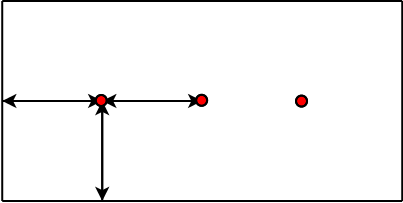
\includegraphics[width=0.4\textwidth]{tavlingssal.png}
\caption{An illustration of an optimal solution for Sample Input 1.}
\label{overflow}
\end{figure}


\section*{Scoring}
Your solution will be tested on a set of test groups. To earn points
for a group, you must pass all test cases in that group.

\begin{tabular}{| l | l | l | l |}
\hline
Group & Points & Constraints & Other\\ \hline
1     & 40         & $ 1 \le N \le 1000 $ & \\ \hline
2     & 30         & $ 1 \le N \le 10^6 $ & \\ \hline
3     & 30         & $ 1 \le N \le 10^9 $ & \\ \hline
\end{tabular}
